\begin{todo}
  Discuss the overall framework, and highlight the major steps and challenges in learning and control.
\end{todo}

\begin{figure}[!t]
  \centering
  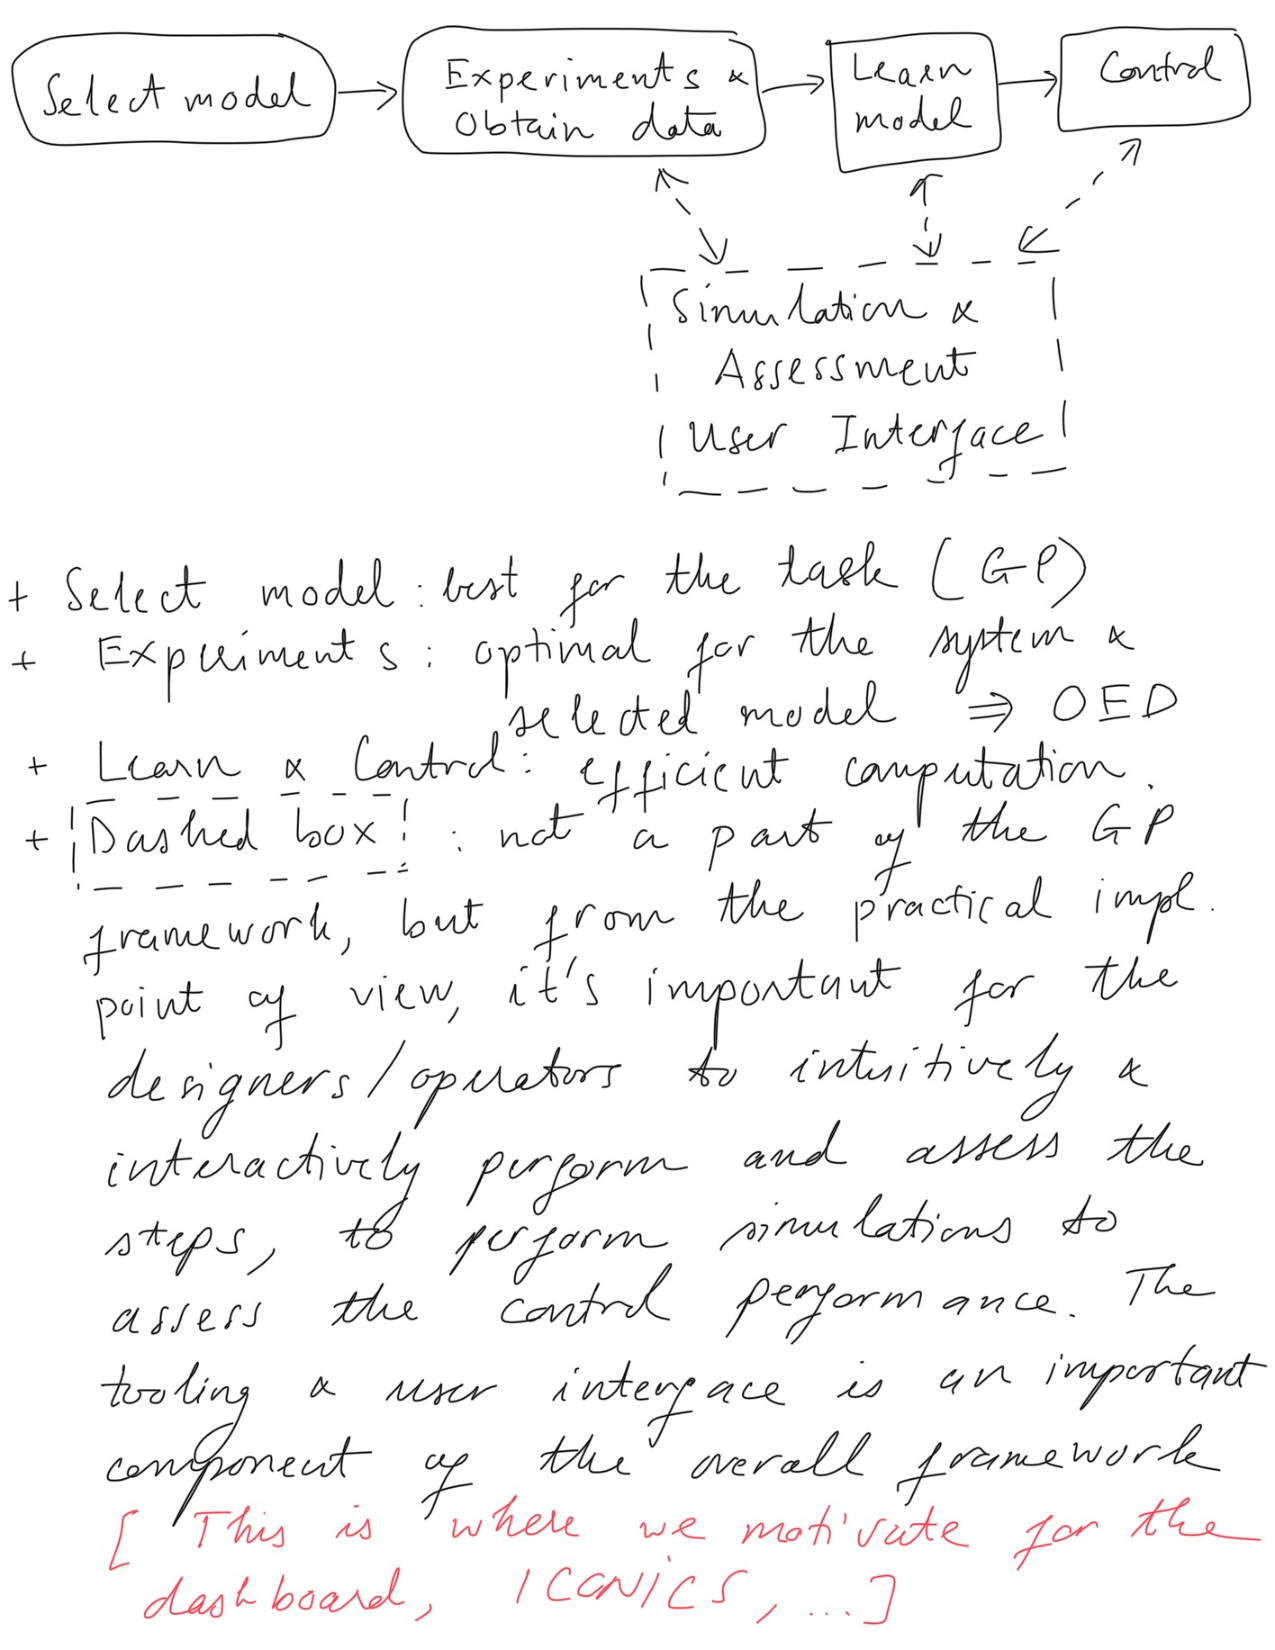
\includegraphics[width=\columnwidth]{overall}
  \caption{Components of the framework, addressing the major steps of data-driven predictive control development: modeling, control synthesis, and simulation-assessment-deployment.}
  \label{fig:overall}
\end{figure}

The development of a data-driven predictive controller for any physical system generally follows these steps:
\begin{enumerate}
\item Establish the control goals and specifications, identify the variables to be controlled.
\item Obtain a data-driven model of the physical system. 
\item Formulate a predictive controller using the learned model.
\item Simulate and assess the performance of the closed-loop control system.
\item If the specifications are met, deploy the controller.
\end{enumerate}

A framework that addresses the last four steps of this development process is presented in this paper.
Figure~\ref{fig:overall} illustrates the major components of our framework, briefly described below and detailed in the subsequent sections.
\begin{enumerate}
\item \textbf{Model type selection:} An appropriate type of control-oriented models must be selected to capture the interested behaviors of the physical system.
  There are basically two types of such data-driven models.  One can \emph{mix black-box and physics-based models} by using machine learning to learn only the dynamics of a sub-system or to model uncertainties in the dynamics while the rest of the system is based on physical principles.
  Alternatively, a \emph{fully black-box model} may be developed, in which the full system dynamics of interest is modeled purely from data using machine learning.  Even then, a black-box model may incorporate domain insights and physical characteristics of the system, for examply by selecting a suitable structure of the machine learning model.
  Our work focuses on the black-box approach to overcome the major challenge of expensive modeling process for buildings, as discussed earlier in section~\ref{sec:introduction}.
  In particular, we choose to model buildings with Gaussian Processes, see Sections~\ref{sec:modeling:gp} and \ref{sec:modeling:building}, for their flexibility and their ability to work well with small data and to provide predictive uncertainty information.
\item \textbf{Experiments:} To learn a model of a physical system from data, experiments are typically performed to excite the system behaviors of interest, so that relevant data can be obtained.
  The quality of the training data is crucial to the quality of the model. 
  However, in practice, historical data that are available from complex systems like buildings are usually based on rule-based controllers, hence they might be insufficient to explain the relationship between the inputs and the outputs of the system.
  Furthermore, the amount and quality of training data we can practically obtain is usually limited due to many factors such as a short permitted duration for experiments and operational or safety constraints of the physical system.
  For example, in buildings, experiments are limited by the short time window during which various energy control set-points are allowed to change, and by the allowable ranges of values and ramp rates of these set-points.
  To learn an optimal model for a specific purpose, it is therefore desirable to design the experiments so that the data quality is maximized, in the sense that the model obtained from the data with a specific learning technique likely has the best quality possible.
  In Section~\ref{sec:modeling:oed}, we present a method for \emph{optimal experiment design} (OED) using Gaussian Processes, which sequentially generates control inputs that result in high quality training data for data-driven modeling.
\item \textbf{Model training:} This step trains a model of the system on the obtained data.
\item \textbf{Control synthesis:} The obtained model is incorporated in an optimization formulation that seeks to minimize a certain cost function, depending on the application, while maintaining operational and safety constraints.
  % There are two major challenges here.
  % First, many data-driven models, including the Gaussian Processes used in this work, are non-convex and sometimes non-differentiable, resulting in high computational complexity of the optimization.
  % Second, it is difficult to guarantee the desirable performance and robustness of a control system with a black-box model due to the model uncertainty.  
  A major challenge of this step is that it is difficult to guarantee the desirable performance and robustness of a control system with a black-box model due to the model uncertainty.  
  However, it is possible to provide probabilistic guarantees with a learning algorithm based on Gaussian Processes, by defining chance constraints or account for model uncertainty in the cost while solving the optimization problem.
  This helps bound the performance errors with high confidence. 
\item \textbf{Simulation and deployment:} Efficient implementation of the OED, learning, and control algorithms is an important part of our framework.  In addition, from the practical point of view, it is crucial for the users of our framework to be able to intuitively and interactively perform the above steps, run simulations, assess the control performance, and deploy the controller on an existing Supervisory Control and Data Acquisition (SCADA) system.  Implementation of our framework on a commercial SCADA system is presented in Section~\ref{sec:case-study}.
\end{enumerate}

The overall structure of our framework for building energy systems is summarized in Figure~\ref{fig:overview}.

\begin{figure}[!t]
	\centering
	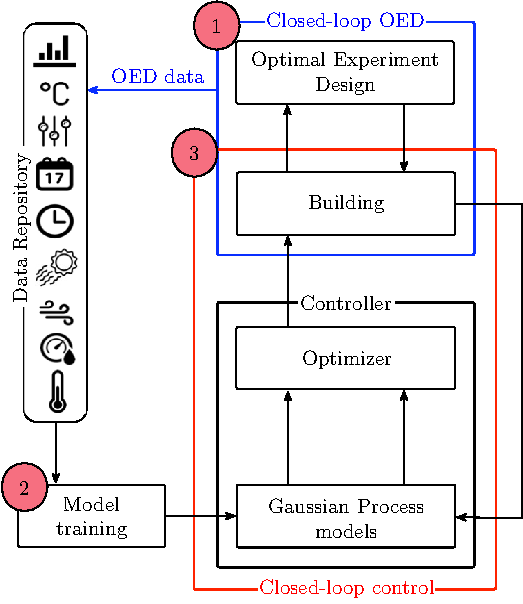
\includegraphics[width=0.9\linewidth]{overview}
	\caption{Overall structure of the framework: (1) Optimal experiment design sequentially samples the inputs and applies to the system to generate training data; (2) Model training learns a model from data; (3) Model Predictive Controller uses a Gaussian Process model learned on the OED data for receding horizon control.}
	\label{fig:overview}
\end{figure}


%%% Local Variables:
%%% mode: latex
%%% TeX-master: "main"
%%% End:
